\chapter{\IfLanguageName{dutch}{Stand van zaken}{State of the art}}
\label{ch:stand-van-zaken}

% Tip: Begin elk hoofdstuk met een paragraaf inleiding die beschrijft hoe
% dit hoofdstuk past binnen het geheel van de bachelorproef. Geef in het
% bijzonder aan wat de link is met het vorige en volgende hoofdstuk.

% Pas na deze inleidende paragraaf komt de eerste sectiehoofding.

%Dit hoofdstuk bevat je literatuurstudie. De inhoud gaat verder op de inleiding, maar zal het onderwerp van de bachelorproef *diepgaand* uitspitten. De bedoeling is dat de lezer na lezing van dit hoofdstuk helemaal op de hoogte is van de huidige stand van zaken (state-of-the-art) in het onderzoeksdomein. Iemand die niet vertrouwd is met het onderwerp, weet nu voldoende om de rest van het verhaal te kunnen volgen, zonder dat die er nog andere informatie moet over opzoeken \autocite{Pollefliet2011}.
%
%Je verwijst bij elke bewering die je doet, vakterm die je introduceert, enz. naar je bronnen. In \LaTeX{} kan dat met het commando \texttt{$\backslash${textcite\{\}}} of \texttt{$\backslash${autocite\{\}}}. Als argument van het commando geef je de ``sleutel'' van een ``record'' in een bibliografische databank in het Bib\LaTeX{}-formaat (een tekstbestand). Als je expliciet naar de auteur verwijst in de zin, gebruik je \texttt{$\backslash${}textcite\{\}}.
%Soms wil je de auteur niet expliciet vernoemen, dan gebruik je \texttt{$\backslash${}autocite\{\}}. In de volgende paragraaf een voorbeeld van elk.
%
%\textcite{Knuth1998} schreef een van de standaardwerken over sorteer- en zoekalgoritmen. Experten zijn het erover eens dat cloud computing een interessante opportuniteit vormen, zowel voor gebruikers als voor dienstverleners op vlak van informatietechnologie~\autocite{Creeger2009}.

In vorig hoodstuk werd Flutter kort geïntroduceerd als een veelomvattend cross-plaftform framework. In dit hoofdstuk wordt de huidige stand van zaken over Flutter besproken. Aangezien Flutter recentelijk is geïntroduceerd wordt het framework regelmatig geüpdate met nieuwe functies en nieuwigheden. Dit hoofdstuk bouwt verder op die van \autocite{Coninck2019}, daarnaast wordt het concept State Management uitvoerig besproken. Tenslotte bekijken we State Management in Flutter en de verschillende mogelijkheden. 
\newline

\section{Flutter}
\subsection{Populariteit van Flutter}
Flutter is een UI toolkit van Google voor het bouwen van native gecompileerde applicaties voor mobiel, web en desktop vanuit één enkele codebase. Doordat Flutter meerdere platformen kan bereiken met slechts één codebase kreeg het de nodige interesse van bedrijven. Vanuit het standpunt van de bedrijven zijn er heel wat kosten uit te sparen.

Flutter kenmerkt zich vooral door de snelle ontwikkelingsomgeving. Mede dankzij de \emph{Stateful Hot Reload} en de reeds tal van beschikbare widgets. Stateful Hot Reload zorgt ervoor dat de nieuwe broncode geïnjecteerd wordt in de Dart Virtual Machine (VM), waardoor het Flutter framework zich automatisch herbouwt, dit zorgt ervoor dat wijzigingen direct zichtbaar zijn in de applicatie. Op de officiële website van Flutter worden er tal van widgets aangeboden, zoals een invoerveld, knop... Dit weerhoudt de ontwikkelaar niet om deze widgets naar zijn behoefte zonodig aan te passen.

Een tweede kenmerk van Flutter is dat de eindapplicaties Native Performance aanbieden voor de eindgebruiker. Flutter compileert de broncode naar native ARM machine code door gebruik van de Dart Native Compilers \autocite{Dart}.

Flutter is een open-source project, gepubliceerd door Google waardoor het beroep kan doen op de nodige financiële noden om het framework te laten groeien. 

Deze literatuurstudie is gebaseerd op de bachelorproef van \autocite{Coninck2019}

\subsection{Alles is een widget}
Het kernprincipe van Flutter is dat alles een widget is. Een widget is als het ware een bouwsteen van een applicatie. Zoals reeds gezegd alles is een widget, zo zijn een knop, een lettertype en een kleur allemaal widgets. 

Een widget wordt beschouwd als een component van een groter geheel, waarbij elke widget zijn specifiek doel heeft.
Hoofdzakelijk zijn er twee soorten widgets te onderscheiden, een Stateless widget en een Stateful widget. Meer uitleg over state in het volgende hoofdstuk. Een voorbeeld van een Stateles widget is een foto, dit soort widget houdt geen interne state bij. Een invoerveld is een voorbeeld van een Stateful widget, deze houdt een interne state bij van de ingevoerde tekst. 
\newline

\subsection{Sterktes van Flutter}
Een Flutter applicatie wordt geschreven in de taal Dart, meer over de programmeertaal Dart in volgende sectie. Kort samengevat wordt de geschreven Dart code gecompileerd in de native ARM en x86 code. 
Dit zorgt ervoor dat de applicatie volledige toegang heeft tot de apparaat services, zoals Bluetooth en camera
Dit wil zeggen dat de applicatie met native prestaties op de apparaten gebruikt kan worden.


\begin{figure}
    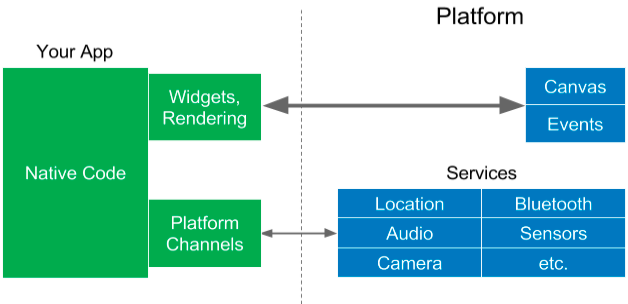
\includegraphics[width=\linewidth]{img/stand-van-zaken/flutter-app-architecture.png}
    \caption{De architectuur van een Flutter applicatie}
    \label{fig:flutter-app-architecture}
\end{figure}

Nadeel is hier dat een ontwikkelaar dezelfde applicatie moet schrijven voor de verschillende platformen aangezien deze andere SDK's (Software Development Kit) hanteren. \autocite{Coninck2019}
\begin{figure}
    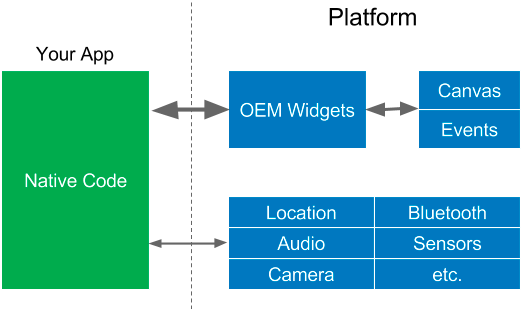
\includegraphics[width=\linewidth]{img/stand-van-zaken/native-app-architecture.png}
    \caption{De architectuur van een native applicatie}
    \label{fig:flutter-app-architecture}
\end{figure}

Andere cross-platform frameworks zoals React Native, maken gebruik van een vertaler. In het geval van React Native is dit de JavaScript Bridge. De geschreven JavaScript code wordt door de JavaScript Bridge omgezet om de native platformen te kunnen aanspreken, zoals te zien op \ref{fig:react-native-app-architecture}  \autocite{Kuitunen2019}

\begin{figure}
    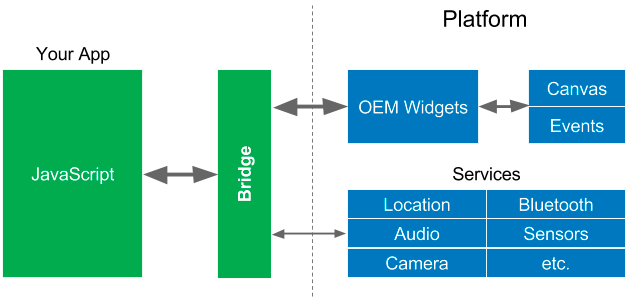
\includegraphics[width=\linewidth]{img/stand-van-zaken/react-native-app-architecture.png}
    \caption{De architectuur van een React Native applicatie}
    \label{fig:react-native-app-architecture}
\end{figure}

% TODO: supported platforms

\subsection{Dart}
De taal die Flutter gebruikt is Dart. De populariteit van deze taal is de laatste tijd gestegen, mede dankzij de populariteit van Flutter.
Dit gedeelte is voornamelijk gebasseerd op een artikel van een Senior Software Engineer bij Google, Wm Leler.

De syntax van Dart is gelijkaardig aan die van Java, C# en Javascript.
Een belangrijke troef van Dart is dat het zowel Ahead Of Time (AOT) als Jus In Time (JIT) gecompileerd kan worden. Het feit dat Dart AOT gecompileerd kan worden heeft als gevolg dat een Flutter applicatie zeer rap en quasi helemaal aangepast kan worden.
De JIT compilatie lost de verwachtignen van elke ontwikkelaar in. De JIT zorgt ervoor dat wijzigingen tijdens het ontwikkelen van de applicatie quasi direct zichtbaar zijn op het apparaat. Dart maakt het mogelijk dat Flutter over Hot Reloading beschikt. \autocite{Leler2017a}
\newline
Op dit moment is de laatste stabiele versie van Dart 2.5.0. Met nieuwe toevoegingen in versie 2.3.0 zoals de spread operator (...) en toekomstzicht op extension methods gaat Dart een mooie toekomst tegemoed. \autocite{Thomsen2019}